\documentclass{beamer}


\mode<presentation>
{
  \usetheme{CambridgeUS}
	\usecolortheme{beaver}
  % or ...

  \setbeamercovered{transparent}
  % or whatever (possibly just delete it)
}


\usepackage{xeCJK}
\usepackage{ulem}
\usepackage[english]{babel}
\usepackage[utf8]{inputenc}
\usepackage{times}
\usepackage[T1]{fontenc}
\usepackage{hyperref}
\usepackage{pifont}
\usepackage{biblatex}
\usepackage{bibentry}
\usepackage{verbatim}
\bibliography{cite}
\newcommand{\cmark}{\ding{51}}%
\newcommand{\xmark}{\ding{55}}%
\setCJKmainfont{WenQuanYi Micro Hei}
\renewcommand{\raggedright}{\leftskip=0pt \rightskip=0pt plus 0cm}
\raggedright

\let\oldfootnotesize\footnotesize
\renewcommand*{\footnotesize}{\oldfootnotesize\tiny}

\title[Intelligent Software Engineering] 
{Intelligent Software Engineering}
\subtitle{Software Testing}

\author[Zhilei Ren] 
{Zhilei Ren}

\institute[Dalian University of Technology] % (optional, but mostly needed)
{
\\
\includegraphics[width=0.1\textwidth]{../utils/logo.png}\\
Dalian University of Technology
}


\subject{Software Engineering}



\pgfdeclareimage[width=0.08\textwidth]{university-logo}{../utils/logo.png}
\logo{\pgfuseimage{university-logo}}



% Delete this, if you do not want the table of contents to pop up at
% the beginning of each subsection:
\AtBeginSubsection[]
{
  \begin{frame}<beamer>{Outline}
    \tableofcontents[currentsection,currentsubsection]
  \end{frame}
}


% If you wish to uncover everything in a step-wise fashion, uncomment
% the following command: 

%\beamerdefaultoverlayspecification{<+->}

\setbeamertemplate{section in toc}[circle]
\setbeamertemplate{items}[circle]
\setbeamertemplate{caption}[numbered]
\setbeamertemplate{bibliography item}{\insertbiblabel}
\setbeamertemplate{bibliography entry title}{}
\setbeamertemplate{bibliography entry journal}{}

\begin{document}

\begin{frame}
  \titlepage
\end{frame}

%\begin{frame}{Outline}
%  \tableofcontents[currentsection,currentsubsection, 
%    hideothersubsections, 
%    sectionstyle=show,
%]
%\end{frame}

\AtBeginSection[]
{
 \begin{frame}<beamer>
 \frametitle{Outline}
 \tableofcontents[currentsection]
 \end{frame}
}
\begin{frame}[t]{bug or feature?}
\end{frame}

\begin{frame}[t]{Fuzz Testing}
In programming and software development, fuzzing or fuzz testing is an automated software testing technique that involves providing invalid, unexpected, or random data as inputs to a computer program. The program is then monitored for exceptions such as crashes, failing built-in code assertions, or potential memory leaks\footnote{\url{https://en.wikipedia.org/wiki/Fuzzing}}.
\end{frame}

\begin{frame}[t]{Differential Testing}
Differential testing, also known as differential fuzzing, is a software testing technique that detect bugs, by providing the same input to a series of similar applications (or to different implementations of the same application), and observing differences in their execution. Differential testing complements traditional software testing because it is well-suited to find semantic or logic bugs that do not exhibit explicit erroneous behaviors like crashes or assertion failures. Differential testing is also called back-to-back testing\footnote{\url{https://en.wikipedia.org/wiki/Differential_testing}}.
\end{frame}


\begin{frame}[t]{Metamorphic Testing}
Metamorphic testing (MT) is a property-based software testing technique, which can be an effective approach for addressing the test oracle problem and test case generation problem. The test oracle problem is the difficulty of determining the expected outcomes of selected test cases or to determine whether the actual outputs agree with the expected outcomes\footnote{\url{https://en.wikipedia.org/wiki/Metamorphic_testing}}.
\end{frame}

\begin{frame}[t]{Metamorphic Testing}
Metamorphic relations (MRs) are necessary properties of the intended functionality of the software, and must involve multiple executions of the software. Consider, for example, a program that implements sin x correct to 100 significant figures; a metamorphic relation for sine functions is $sin (\pi − x) = sin(x)$. Thus, even though the expected value of $sin x_1$ for the source test case $x_1 = 1.234$ correct to the required accuracy is not known, a follow-up test case $x_2 = \pi − 1.234$ can be constructed. We can verify whether the actual outputs produced by the program under test from the source test case and the follow-up test case are consistent with the MR in question. Any inconsistency (after taking rounding errors into consideration) indicates a failure: 31  of the program, caused by a fault: 31  in the implementation.
\end{frame}
\begin{frame}[t]{Differential Testing}
    Differential testing, also known as differential fuzzing, is a software testing technique that detect bugs, by providing the same input to a series of similar applications (or to different implementations of the same application), and observing differences in their execution. Differential testing complements traditional software testing because it is well-suited to find semantic or logic bugs that do not exhibit explicit erroneous behaviors like crashes or assertion failures. Differential testing is also called back-to-back testing\footnote{\url{https://en.wikipedia.org/wiki/Differential_testing}}.
\end{frame}

\begin{frame}[t]{EvoSuite}
    EvoSuite is a tool that automatically generates unit tests for Java software. EvoSuite uses an evolutionary algorithm to generate JUnit tests. EvoSuite can be run from the command line, and it also has plugins to integrate it in Maven, IntelliJ and Eclipse. EvoSuite has been used on more than a hundred open-source software and several industrial systems, finding thousands of potential bugs\footnote{\url{https://en.wikipedia.org/wiki/EvoSuite}}.
\end{frame}

\begin{frame}[t]{Evolutionary Fuzz Testing}
    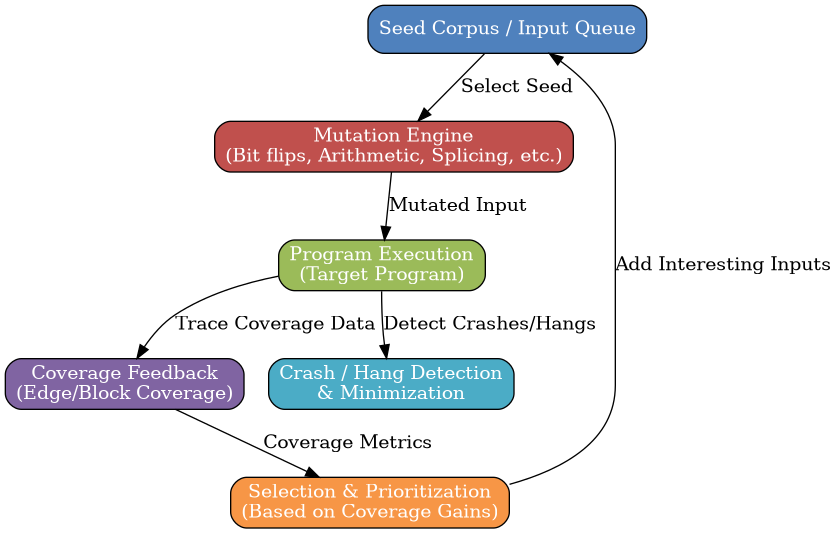
\includegraphics[width=.5\textwidth]{evo_fuzz.png} 
\end{frame}

\begin{frame}
\frametitle{Main Modules Description}
 
\begin{itemize}
    \item \textbf{Seed Corpus / Input Queue (Blue)}
    \begin{itemize}
        \item Holds the initial set of seed inputs and manages the queue of inputs waiting to be processed.
    \end{itemize}
    
    \item \textbf{Mutation Engine (Red)}
    \begin{itemize}
        \item Generates new test inputs by applying mutation strategies (e.g., bit flips, arithmetic operations, splicing).
    \end{itemize}
    
    \item \textbf{Program Execution (Green)}
    \begin{itemize}
        \item Executes the target program using mutated inputs, collects trace coverage data, and monitors for crashes or hangs.
    \end{itemize}
    
    \item \textbf{Crash / Hang Detection \& Minimization (Cyan)}
    \begin{itemize}
        \item Detects crashes or hangs during execution and minimizes the problematic inputs for debugging.
    \end{itemize}
    
    \item \textbf{Coverage Feedback (Purple)}
    \begin{itemize}
        \item Collects data on which parts of the program were exercised by the inputs to guide the fuzzing process.
    \end{itemize}
    
    \item \textbf{Selection \& Prioritization (Orange)}
    \begin{itemize}
        \item Selects and prioritizes inputs based on coverage metrics to discover new paths or trigger crashes.
    \end{itemize}
\end{itemize}
 
\end{frame}
 
\begin{frame}
\frametitle{Overall Flow}
 
\begin{enumerate}
    \item \textbf{Initialization}
    \begin{itemize}
        \item Start with a seed corpus or input queue containing initial test inputs.
    \end{itemize}
    
    \item \textbf{Mutation}
    \begin{itemize}
        \item Select seeds from the input queue and apply mutation strategies to generate new inputs.
    \end{itemize}
    
    \item \textbf{Execution}
    \begin{itemize}
        \item Execute the target program with mutated inputs, collect coverage data, and detect crashes or hangs.
    \end{itemize}
    
    \item \textbf{Detection and Minimization}
    \begin{itemize}
        \item Record detected crashes or hangs and minimize the inputs for debugging.
    \end{itemize}
    
    \item \textbf{Feedback and Prioritization}
    \begin{itemize}
        \item Use coverage feedback to evaluate inputs, select and prioritize those that improve coverage.
    \end{itemize}
    
    \item \textbf{Iteration}
    \begin{itemize}
        \item Iterate the process, refining inputs based on coverage feedback to maximize code exploration and crash discovery.
    \end{itemize}
\end{enumerate}
 
\end{frame}
\end{document}

